\documentclass{beamer}
%[aspectratio=169]   \usepackage[czech]{babel}
\usepackage{apo-lecture-cz}
\usepackage{pdfpages}
\usepackage{pdfcomment}
\usepackage{listings}
\usepackage{array,multirow}

\subtitle{Lekce 07. Vstup a výstup}
\author{Pavel Píša \phantom{xxxxxxxxx} Petr Štěpán \\ \small\texttt{pisa@fel.cvut.cz}\phantom{xxxx}\small\texttt{stepan@fel.cvut.cz}}
\begin{document}

\maketitle

\section{Vstupy a výstupy}

\begin{frame}
\frametitle{Cíl dnešní přednášky}

\begin{itemize}
 \item Projít, jaké jsou možnosti vstupu a výstupu v počítači
 \item Periférie mapované do paměti
 \item Příklady v QtRvSim
 \item PCI a PCIe sběrnice
\end{itemize}
\end{frame}


\begin{frame}[shrink=10]
\frametitle{Architektura počítače -- John von Neumann}
\begin{center}
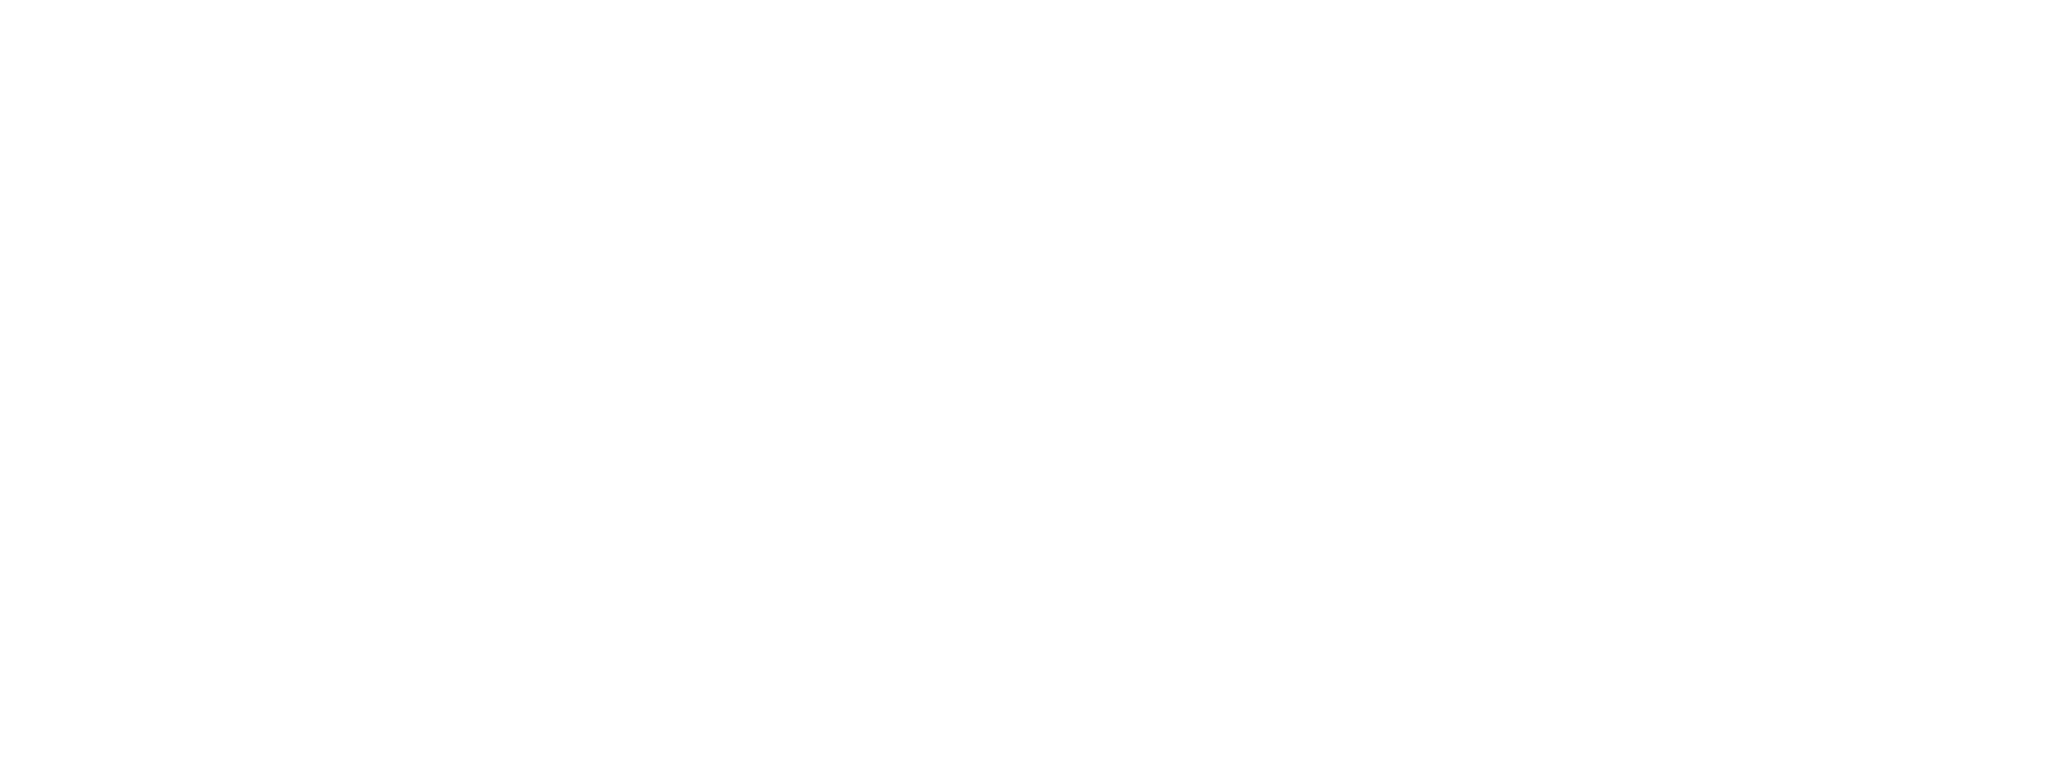
\includegraphics[width=0.5\textwidth]{cpu-vonNeumann.pdf}
\hfill
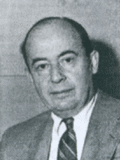
\includegraphics[width=0.15\textwidth]{fig/vonNeumann.png}
\end{center}
\begin{itemize}
\item 5 základních jednotek – řídicí jednotka, aritmeticko-logická jednotka, paměť, vstup (vstupní zařízení), výstup (výstupní zařízení)
\item Architektura počítače by neměla být závislá na řešené úloze, měla by umět provádět program uložený v paměti. Program řídí, co počítač vykonává za instrukce a tím jaké dostane výsledky.
\item Program a data jsou uložena ve stejné paměti, složené z buněk (jednotek) stejné velikosti. Oproti tomu Harvardská architektura měla jeden typ paměti pro program a jiný typ paměti pro data.
\item Další instrukce, která se bude vykonávat je uložena v následující buňce paměti (mimo skoků v programu)
\item Instrukce provádějí aritmetické a logické operace, přesuny dat z/do paměti, skoky a větvení programu a speciální řídicí instrukce.
\end{itemize}
\end{frame}


\begin{frame}
\frametitle{Klasifikace periférií}
Chování:
\begin{itemize}
\item jenom vstup
\item jenom výstup
\item vstup i výstup (v současnosti většina zařízení, i klávesnice má výstup signalizace led)
\end{itemize}

Připojení:
\begin{itemize}
\item přímé propojení CPU a periférie
\item hierarchické -- propojení přes jiné periférie (bridge, switch)
\end{itemize}

Partner:
\begin{itemize}
\item člověk -- jiné parametry komunikace
\item počítač -- většinou rychlejší komunikace
\item prostředí -- senzory a aktuátory
\end{itemize}

Parametry přenosu:
\begin{itemize}
\item kapacita přenosové linky -- maximální možnosti přenosu dat
\item latence -- čas, do kterého se provede přenos dat
\end{itemize}
\end{frame}

\begin{frame}
\frametitle{Klasifikace periférií}

Příklady periférií komunikujících s lidmi:
\begin{itemize}
\item klávesnice -- sice jen vstup, ale moderní často i výstup led diody, velmi malá přenosová rychlost, latence až do 200ms (mimo hraní her) 
\item mikrofon/reproduktory -- přenosová rychlost až 8Mb/s, latence záleží na aplikaci, pro interaktivní komunikaci se vyžaduje latence menší 500 ms, optimálně 150 -- 300 ms 
\item tiskárny/scanery -- přenosová rychlost podle připojení, na latency nezáleží (v řádech vteřin/minut)
\end{itemize}

Příklady periférií pro komunikaci mezi počítači
\begin{itemize}
\item modem -- první modemy 115,2kb/s, LTE max 300 Mb/s, 5G až 500Mb/s
\item sítě/WLAN -- od 10 Mb/s přes 1Gb/s až po 1Tb/s
\item datová úložistě -- HDD, SSD, magnetopáskové jednotky, rychlosti komunikace podle připojení (dnes později), latence SSD nejlepší, HDD horší, magnetopáskové jednotky -- použitelně pouze sekvenční zápis.
\end{itemize}

\end{frame}


\begin{frame}
\frametitle{Klasifikace periférií}

Příklady senzorů a aktuátorů:
\begin{itemize}
\item kamera, laserové hloubkoměry -- rychlosti komunikace podle druhu připojení
\begin{itemize}
\item USB 2.0 max 480 Mb/s, 
\item USB 3.1 max 5Gb/s, 
\item WLAN až 10Gb/s
\end{itemize}
\item aktuátory -- motory DC/PMSM 
\begin{itemize}
\item není důležitá rychlost přenosu, ale latence
\item latence je nejdůležitější parametr pro řízení
\item DC -- latence 0.5-0.05ms, 
\item PMSM -- latence 0.05-0.01ms
\end{itemize}
\end{itemize}

\end{frame}




\begin{frame}
\frametitle{Návrh CPU z přednášky 5}
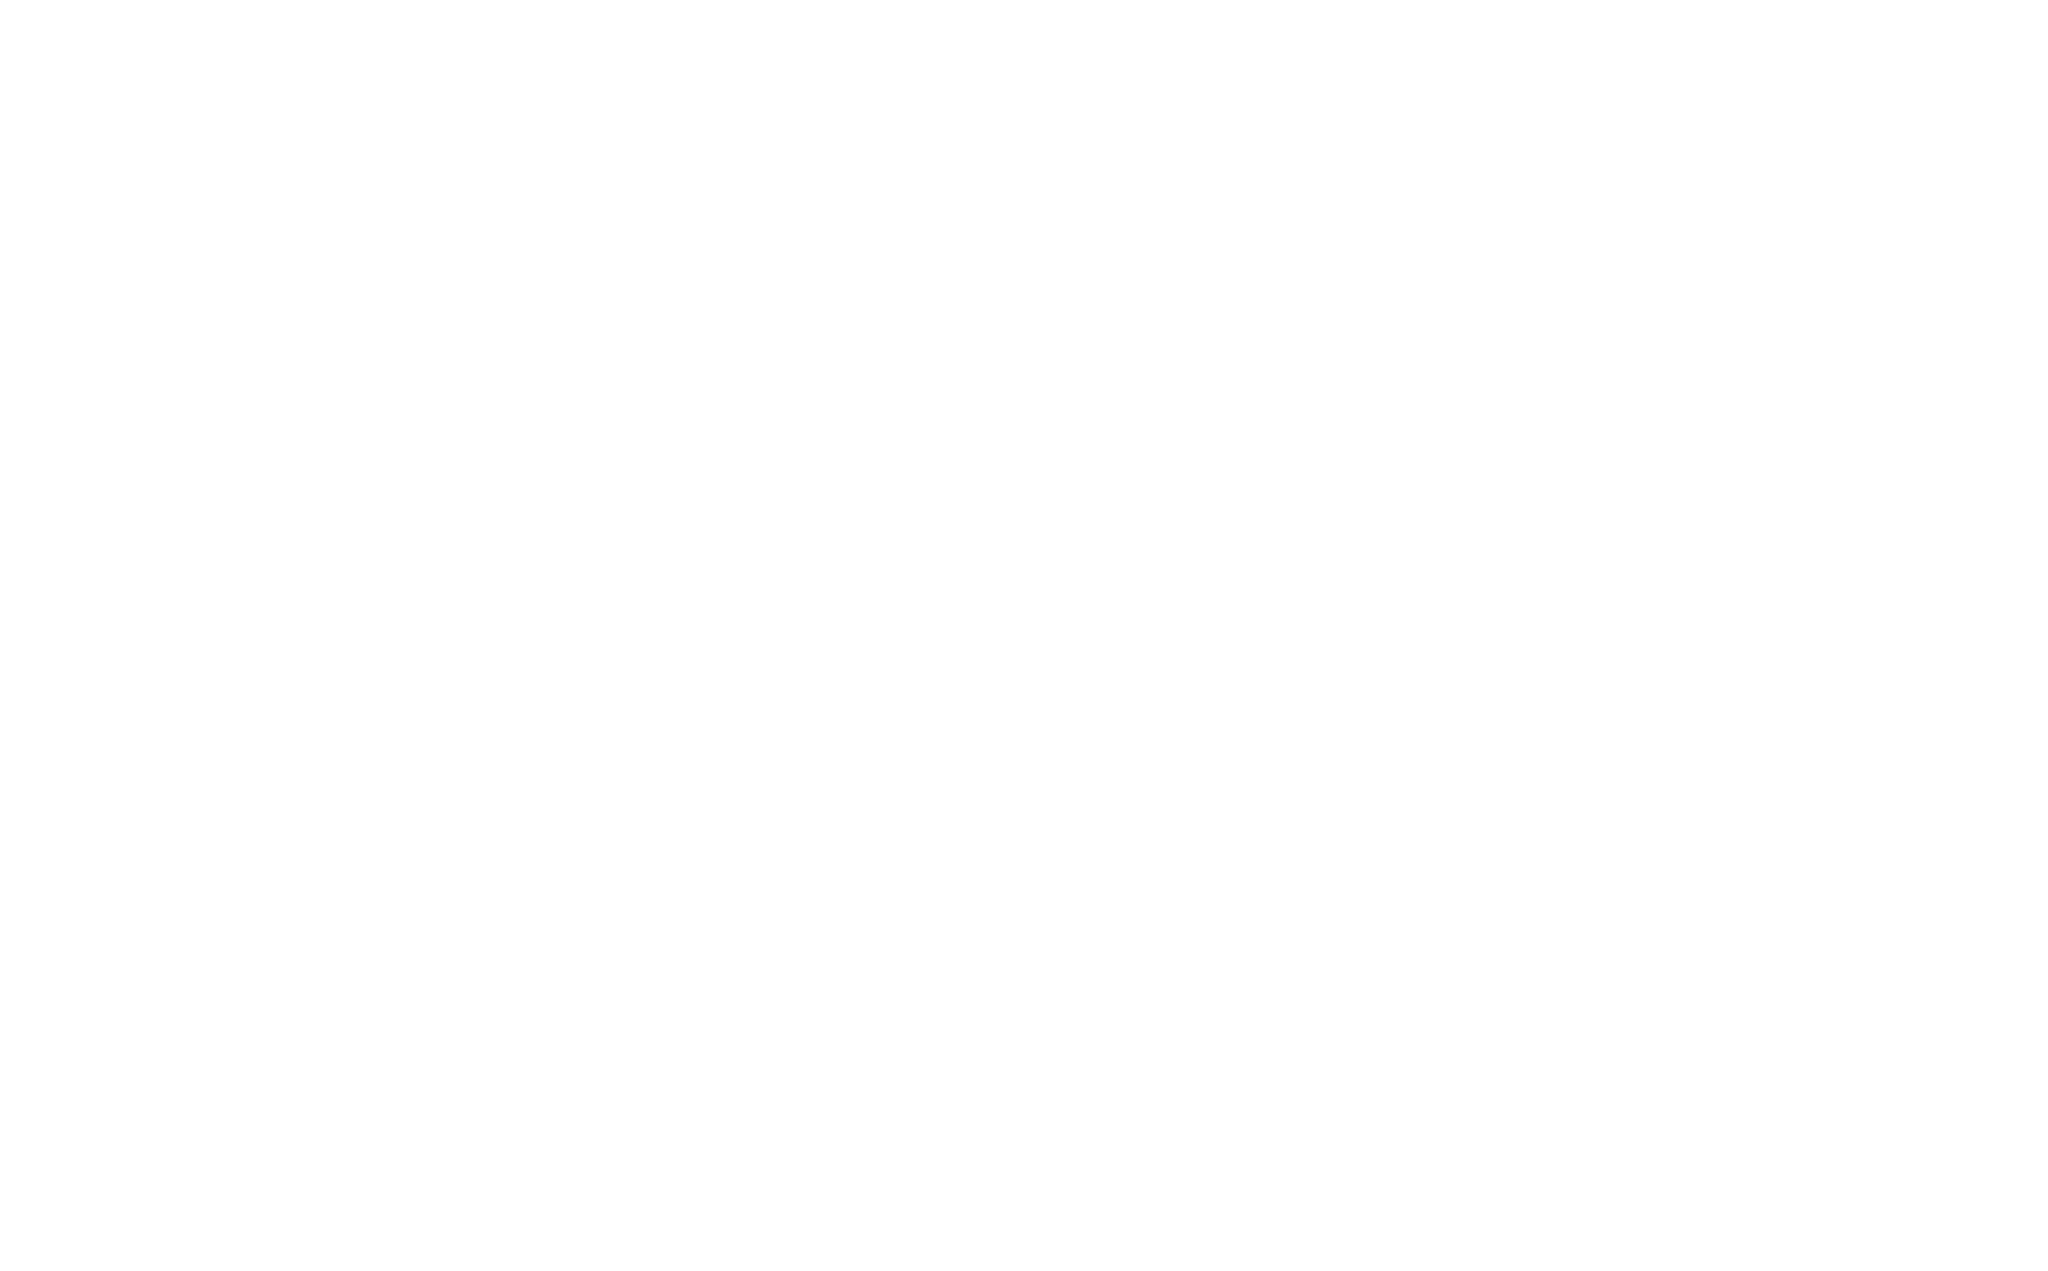
\includegraphics[width=0.95\textwidth]{cpu_design2.pdf}
\end{frame}

\begin{frame}
\frametitle{Propojení CPU s pamětí a perifériemi}
\begin{columns}
\begin{column}{0.4\textwidth}
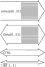
\includegraphics[width=0.9\textwidth]{bus_arch-cz.pdf}
\end{column}
\begin{column}{0.6\textwidth}  
\begin{itemize}
\item Adresová sběrnice (A0..A31) může být oddělená, nebo multiplexovaná, nebo sdílet stejné signály jako datová část
\item Datová sběrnice (D0..D31) může být obousměrná, nebo oddělená pro každý směr zvlášť, paralelní nebo sériová
\begin{itemize}
\item zde na obrázku je paralelní 32-bitová sběrnice typu half-duplex stejné vodiče pro oba směry
\end{itemize}
\item Řídicí signály sběrnice
\begin{itemize}
\item řídí komunikaci na sběrnici, co se bude kam přenášet, kdy přenos začne skončí, pozdrží.
\end{itemize}
\item BE0 to 3 -- pokud je povoleno čtení bajtů na sběrnici širší než 8 bitů.
\end{itemize}
\end{column}
\end{columns}
\end{frame}



\begin{frame}
\frametitle{Přístup CPU k periférii}

Prakticky existují dva různé přístupy:
\begin{itemize}
\item Speciální instrukce 
\begin{itemize}
\item x86 používá instrukce \texttt{in}, \texttt{out}.
\item Tyto instrukce mají podobný formát jako přístup do paměti, ale data čtou a zapisují na sběrnici kde jsou připojeny periférie.
\item Implementace těchto instrukcí potřebuje přístup k jiným sběrnicím.
\item Tyto instrukce se ukázaly neefektivní, nesystematické a moderní periférie je nepoužívají.
\end{itemize}
\item Vyhrazení části adresového prostoru
\begin{itemize}
\item RISC-V nemá speciální instrukce pro komunikace s perifériemi, a proto využívá metodu, že čtení a zápis do určených oblastí paměti vede k čtení a zápisu z periferií.
\item Tento přístup je velmi jednoduše konfigurovatelný, periférie při inicializaci získají paměťový rozsah, který slouží k přesunu dat mezi CPU a perifériemi.
\end{itemize}
\end{itemize}
\end{frame}


\begin{frame}
\frametitle{Paměťově mapované periférie}

\begin{itemize}
\item RISC-V nemá speciální instrukce pro komunikace s perifériemi
\item pro komunikaci s perifériemi se využívá ukládání a čtení z paměti
\item Address Decoder -- rozhoduje, kam se data přesměrují
\end{itemize}
\begin{center}
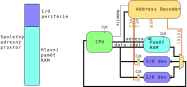
\includegraphics[width=0.88\textwidth]{address_decoder-cz.pdf}
\end{center}
\end{frame}


\begin{frame}
\frametitle{Typy adresových dekodérů}

Centralizovaný dekodér

\begin{center}
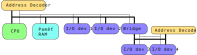
\includegraphics[width=0.8\textwidth]{central-cz.pdf}
\end{center}

Decentralizovaný -- autonomní dekodér

\begin{center}
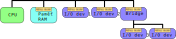
\includegraphics[width=0.8\textwidth]{distributed-cz.pdf}
\end{center}
\end{frame}



\begin{frame}
\frametitle{Způsoby komunikace s periférií}
Data pouze na dotaz:
\begin{itemize}
\item zařízení čeká, až ho CPU osloví a zašle data na výstup, nebo požádá o připravená data ze vstupu
\item pomalejší komunikace, CPU musí aktivně zjišťovat, zda jsou připravená data k příjmu
\end{itemize}

Periférie využívá přerušení k signalizaci svého stavu:
\begin{itemize}
\item pokud dojde ke změně stavu, periférie vyvolá přerušení (přednáška 9)
\item CPU pak aktivně čte, nebo zapisuje data na periférii
\end{itemize}

Periférie využívá přímý přístup do paměti:
\begin{itemize}
\item využívá také přerušení
\item CPU nastaví pouze z/do jaké adresy v paměti se data budou číst/zapisovat a periférie sama řídí přenos dat
\item po ukončení periférie vyvolá přerušení a CPU zkontroluje výsledek přenosu (zda bylo vše v pořádku, nebo došlo k chybě)
\end{itemize}

\end{frame}

\begin{frame}
\frametitle{Zpracování periférií -- Linux (zjednodušeno)}
\begin{columns}
\begin{column}{0.4\textwidth}
Programy komunikují s periferiemi pomocí operačního systému a systémového volání a ovladačů periferií(přehled v přednášce 10, podrobně v předmětu OSY).

\bigskip
Další možností je komunikace přes sdílenou paměť -- náplň dnešní přednášky.
\end{column}
\begin{column}{0.58\textwidth}  
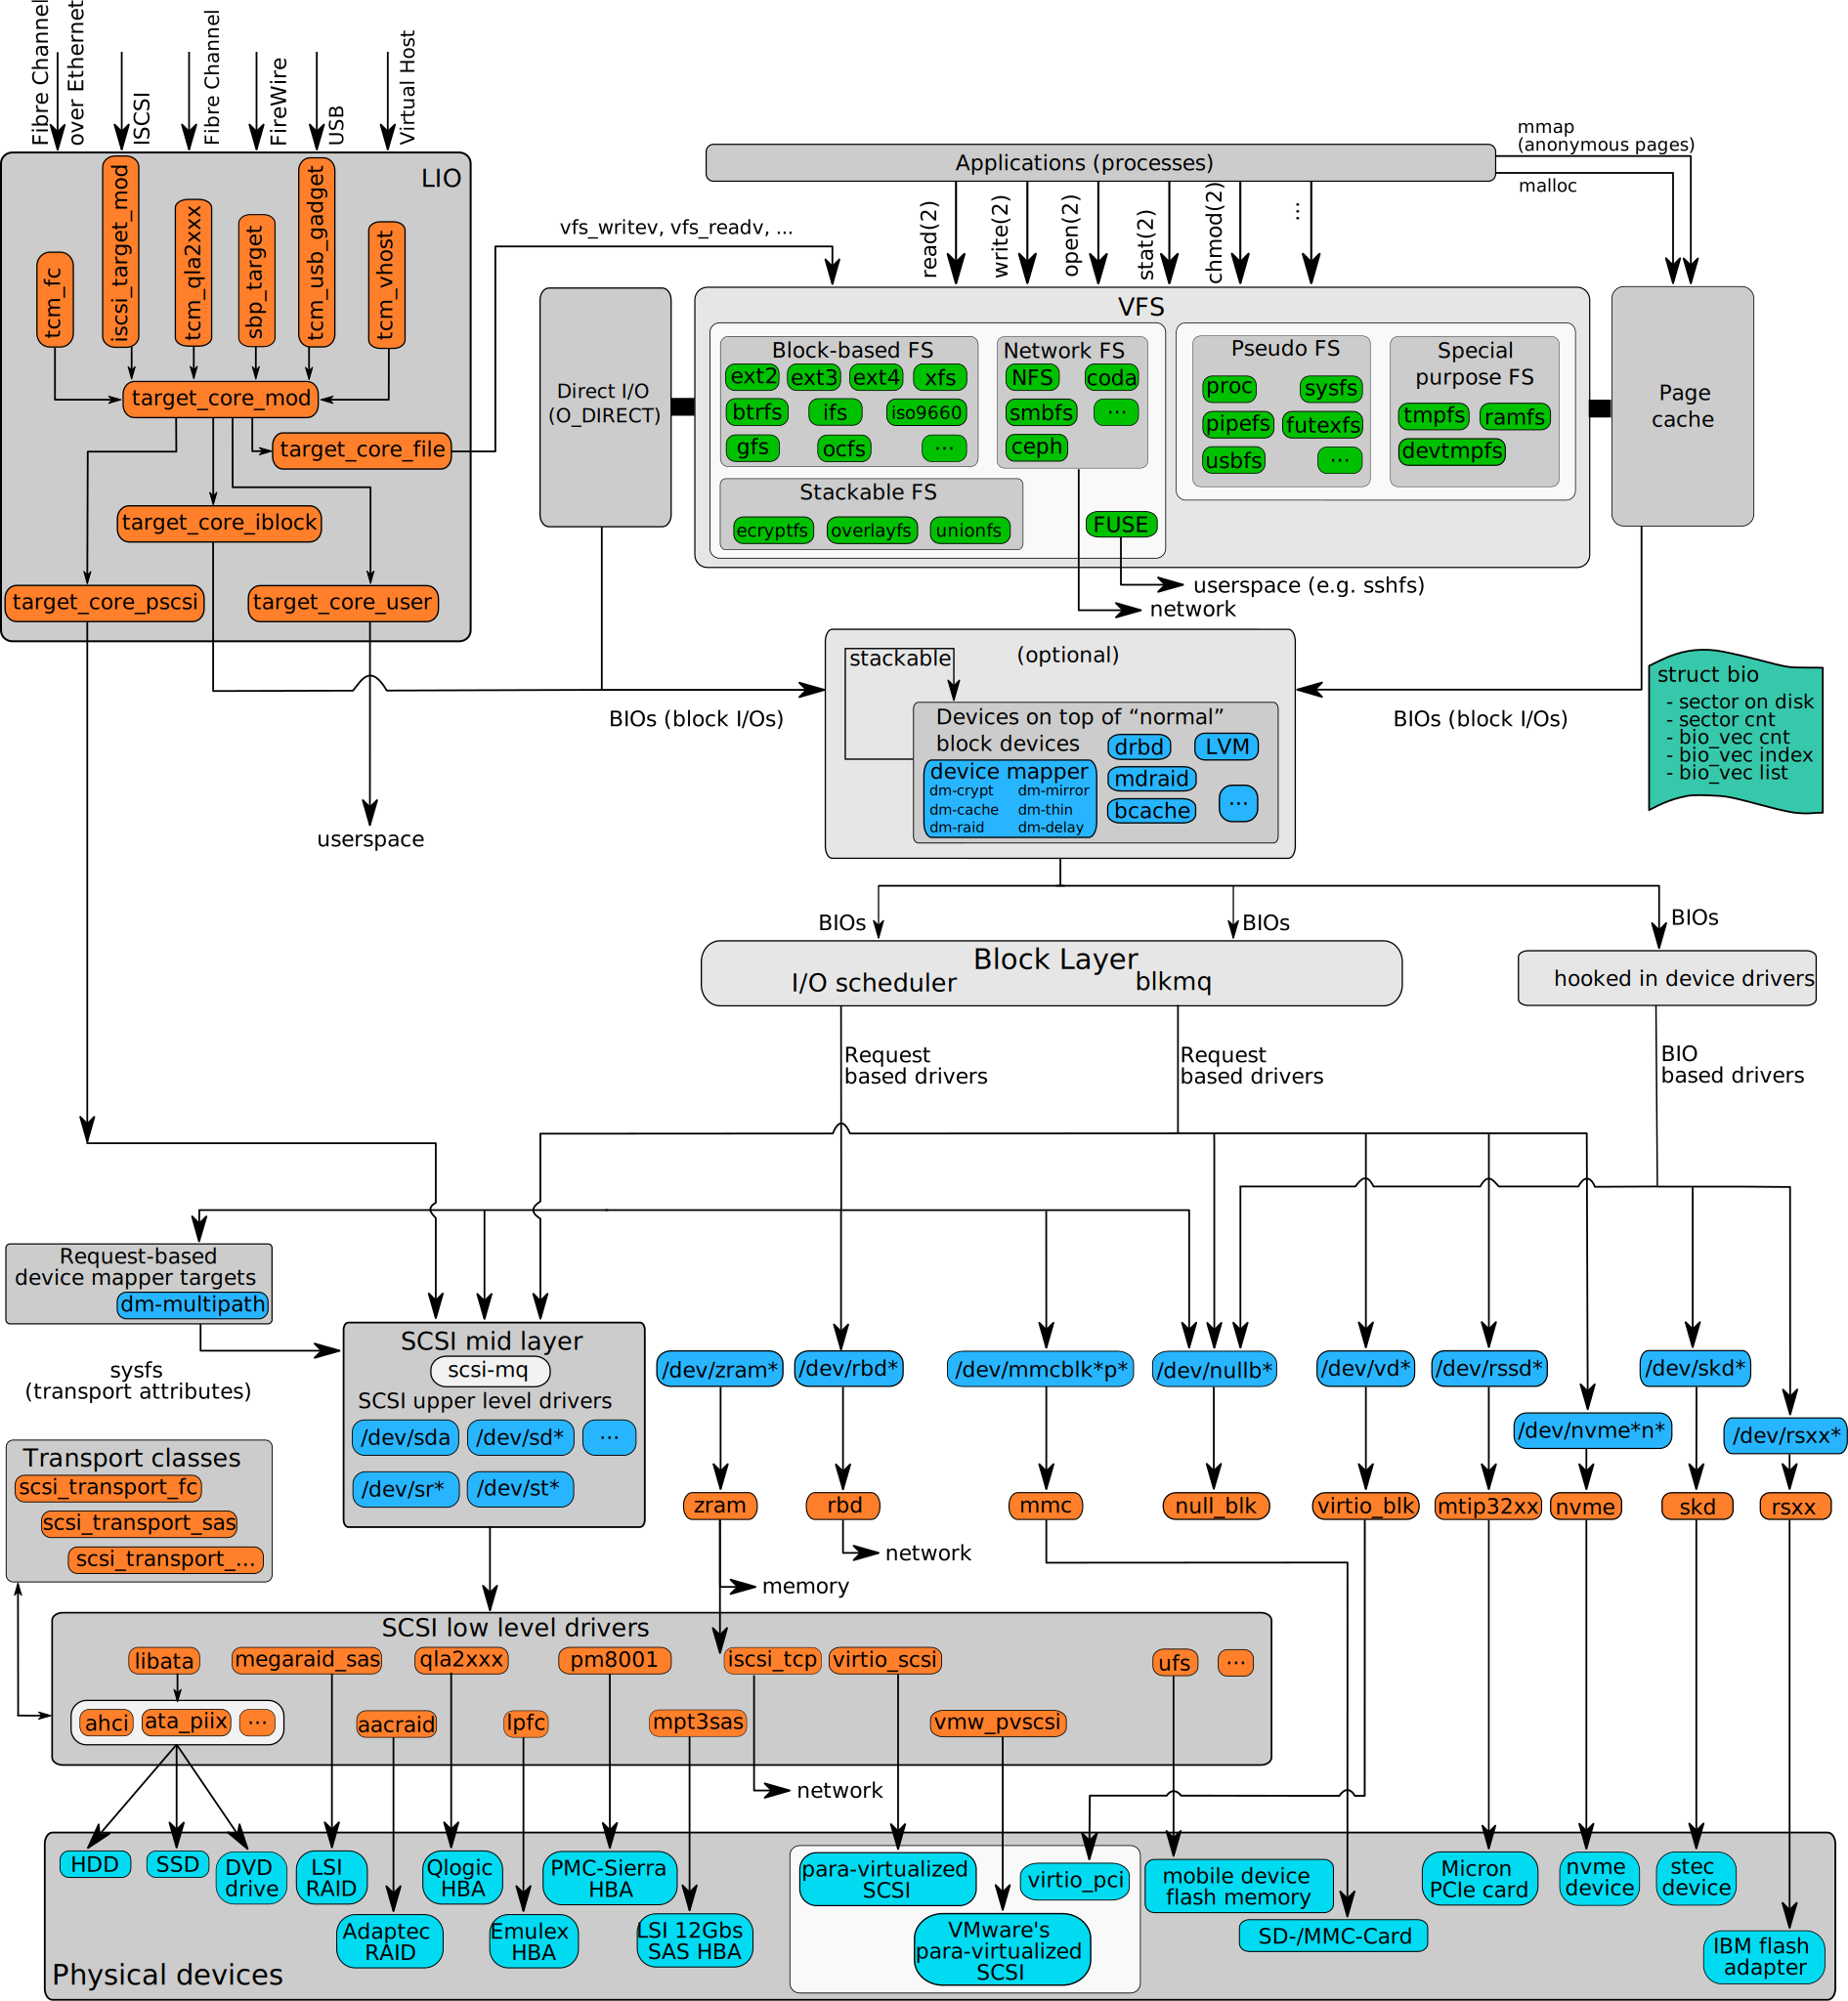
\includegraphics[width=\textwidth]{linux.pdf}
\end{column}
\end{columns}
\end{frame}


\begin{frame}
\frametitle{Systémová volání}

Systémová volání:
\begin{itemize}
\item pro normální uživatele jsou systémová volání zabalená ve funkcích knihovny libc -- POSIX API
\item funkce open
    \begin{itemize}
    \item pro každou periferii lze vytvořit virtuální soubor
    \item tento soubor slouží ke komunikaci s periferií
    \end{itemize}
\item funkce read 
    \begin{itemize}
    \item přečte data od periférie jako by je četlo ze souboru
    \item blokující čtení
        \begin{itemize}
        \item pokud nejsou data funkce read čeká na jejich příchod
        \item při čekání je proces uspán a nezatěžuje CPU
        \end{itemize}
    \item neblokující čtení
        \begin{itemize}
        \item pokud nejsou data, funkce read vrátí zápornou hodnotu 
        \item koordinace čtení je ovládána procesem
        \item data z periférie jsou ukládána nezávisle ovladačem do vnitřních systémových bufferů
        \end{itemize}
    \end{itemize}
\end{itemize}
\end{frame}





\begin{frame}
\frametitle{Kvíz čtení dat}

Funkce scanf čte standardní vstup metodou, že pokud aktuálně nejsou data k dispozici tak se:
\begin{itemize}
\item[A] v cyklu neustále dotazuje, zda jsou data připravena 
\item[B] proces uspí a je nutné ho restartovat
\item[C] proces uspí a operační systém ho probudí, když data přijdou
\item[D] funkce vrátí s hodnotou -1
\end{itemize}
\end{frame}



\section{Periférie v QtRvSim}

\begin{frame}
\frametitle{QtRvSim -- otočné voliče, RGB led}

\begin{itemize}
\item stejný formát dat pro RGB led i načtení tří otočných voličů 
\begin{itemize}
\item bity 24 -- 31 nejsou pro RGB led použity
\end{itemize}
\end{itemize}

\begin{table}
\scriptsize
\begin{tabular}{|m{1.0cm}|m{1.1cm}|m{0.5cm}|m{0.5cm}|m{0.5cm}|m{1.1cm}|m{1.1cm}|m{1.1cm}|}\hline
Bity & 31 ... 27 & 26 & 25 & 24 & 23 ... 16 & 15 ... 8 & 7 ... 0 \\ \hline
Význam & nepoužito & stisk červené & stisk zelené & stisk mod- ré & hodnota červené & hodnota zelené & hodnota modré \\ \hline
\end{tabular}
\end{table}


\begin{itemize}
\item každá jednotlivá RGB led má svoji adresu pro zápis, všechny tři voliče mají svojí adresu pro čtení
\item zápisem pro adresu RGB led se "okamžitě" rozsvítí zadanými hodnotami
\item čtením z adresy otočných voličů se čte jejich stav v aktuálním okamžiku
\end{itemize}

\end{frame}


\begin{frame}[fragile]
\frametitle{QtRvSim -- otočné voliče, RGB led}

\begin{columns}
\begin{column}{0.6\textwidth}  
\begin{minted}[fontsize=\footnotesize]{gas}
#base of SPILED port region
.equ SPILED_REG_BASE,       0xffffc100

#RGB LED 1 barevne slozky – 8 bitu kazda
.equ SPILED_REG_LED_RGB1,   0xffffc110
.equ SPILED_REG_LED_RGB1_o,   0x0010

#RGB LED 2 barevne slozky – 8 bitu kazda
.equ SPILED_REG_LED_RGB2,   0xffffc114
.equ SPILED_REG_LED_RGB2_o,   0x0014

#Tri 8 bitove otocne volice
#nejvyssi bajt informace o stitsknuti
.equ SPILED_REG_KNOBS_8BIT, 0xffffc124 
.equ SPILED_REG_KNOBS_8BIT_o, 0x0024

#32 LEDek kazdy bit jedna LED dioda
.equ SPILED_REG_LED_LINE,   0xffffc104
.equ SPILED_REG_LED_LINE_o,   0x0004
\end{minted}
\end{column}
\begin{column}{0.4\textwidth}
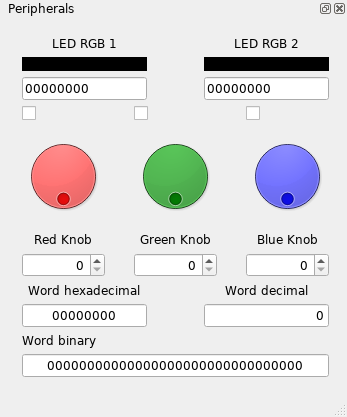
\includegraphics[width=\textwidth]{fig/knobs.png}
\end{column}
\end{columns}

\end{frame}

\begin{frame}[fragile]
\frametitle{Příklad použití informace od otočných voličů}

\begin{minted}[fontsize=\footnotesize]{gas}
    li   a0, SPILED_REG_BASE # a0 ukazuje na zacatek pameti pro I/O
    ori  t2, t2, -1
loop:
    lw   t0, SPILED_REG_KNOBS_8BIT_o(a0)   # nacti data od otocnych volicu
    sw   t0, SPILED_REG_LED_RGB1_o(a0)
    xor  t1, t0, t2
    sw   t1, SPILED_REG_LED_RGB2_o(a0)
    srli t0, t0, 24
    andi t0, t0, 4
    beq  t0, zero, loop    # pokud nebyl zmacknut cerveny volic

    ebreak                    # ukonci program
\end{minted}
\end{frame}

\begin{frame}
\frametitle{Kvíz otočné voliče}

Pokud máme v proměnné \texttt{unsigned int v;} načtené slovo z adresy \texttt{SPILED\_REG\_BASE+SPILED\_REG\_KNOBS\_8BIT\_o} pak informace o stavu zeleného voliče získáme jako:
\begin{itemize}
\item[A] \texttt{((v<<24) \& 0x00ff00)}
\item[B] \texttt{((v>>8) \& 0xff)}
\item[C] \texttt{(v \& 0x30303030)}
\item[D] \texttt{((v>>24) \& 0xf0)}
\end{itemize}
\end{frame}



\begin{frame}
\frametitle{Asynchronní sběrnice vs. synchronní sběrnice}

Asynchronní sběrnice:
\begin{itemize}
\item  dvě základní varianty:
\begin{itemize}
\item Začátek a konec každého bitu je detekovatelný druhou stranou
\item Je dohodnuta doba trvání vyslání jednoho bitu a jednotlivé bajty mají druhou stranou detekovatelný začátek, případně i konec
\end{itemize}
\item Příkladem asynchronní komunikace je sériový port, USB, SATA disky
\end{itemize}


Synchronní sběrnice:
\begin{itemize}
\item Nejjednodušší je vyhradit jeden signál na přenos hodin vysílajícího k přijímajícímu
\item Vyslání data se řídí hodinami, buď jen jedním typem hrany, nebo i na druhý typ hrany
\item Příkladem synchronního přenosu jsou komunikace DDR s pamětí, PCI, PCI Expres
\end{itemize}
\end{frame}


\begin{frame}
\frametitle{Sériová linka}

\footnotesize
Sériová linka (sériový port) je jedna z nejstarších způsobů komunikace využívaných dodnes.
\begin{itemize}
\footnotesize
\item Asynchronní přenos bez hodin.
\item Obě strany jsou nastaveny na stejnou rychlost, která definuje délku vyslání jednoho bitu
\begin{itemize}
\scriptsize
\item Přenos začíná vysláním start bitu (přechod z 1 $\rightarrow$ 0)
\begin{itemize}
\scriptsize
\item Vysláním a příjmem start bitu se synchronizují lokální hodiny všech zařízení
\end{itemize}
\scriptsize
\item Pak se vysílají jednotlivé bity jednoho bajtu
\item Výběrově pak může následovat bit parity pro kontrolu chyb přenosu
\item Poslední je vyslán stop bit (přechod z 0 $\rightarrow$ 1, nebo přidržení 1)
\end{itemize}
\footnotesize
\item Vyslání jednoho bajtu tedy obsahuje vyslání 10-11 bitů
\item Běžné rychlosti, dříve 9600 Bd až 115200 Bd, nově až 921600 Bd (Bd -- Baud = bit per second)
\end{itemize}

\begin{center}
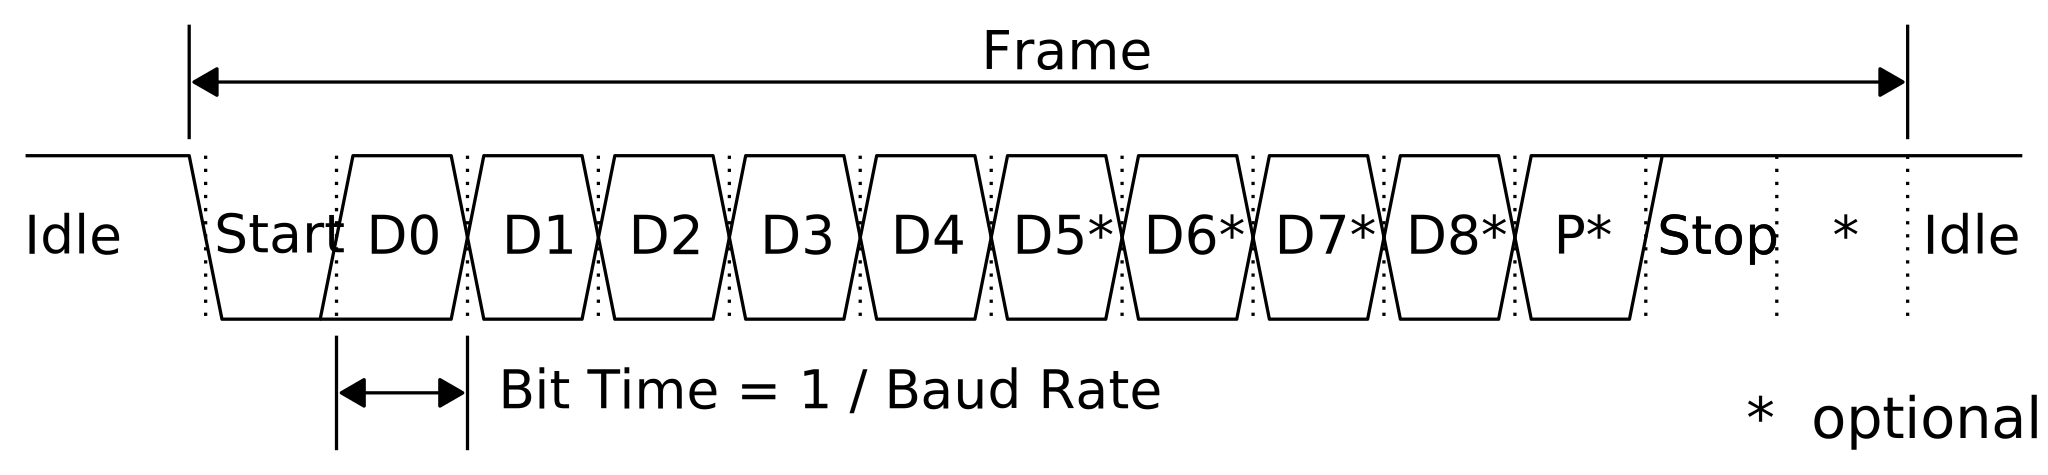
\includegraphics[width=0.8\textwidth]{serial_signals.pdf}
\end{center}
\end{frame}

\begin{frame}[shrink=5]
\frametitle{Sériová linka}

Základní specifikace RS 232:
\begin{itemize}
\item Navrženo pouze pro propojení dvou zařízení
\item Obě zařízení jsou propojené signální zemí
\item 0 reprezentována +3 -- +15V, 1 reprezentuje -3 -- -15 V
\item Plně duplexní, tzn. jiné signály pro přenos tam a jiné pro přenos zpět
\item Mohou být použité signály pro pozdržení vysílání, nebo příjmu při přeplněném lokálním bufferu
\end{itemize}

Základní specifikace RS 422:
\begin{itemize}
\item Plovoucí signál, Rx+, Rx- -- vysílaná hodnota je napětí mezi dvěma vodiči, lze použít až na vzdálenost 1200m
\item Plně duplexní, tzn. jiné signály pro přenos tam a jiné pro přenos zpět
\item Může být více posluchačů pro jednoho vysílajícího
\end{itemize}

Základní specifikace RS 485:
\begin{itemize}
\item Plovoucí signál stejně jako 422
\item Může být half-duplex - tedy pouze dva vodiče, je nutné po vyslání dat odpojit se od sběrnice a poslouchat zda někdo odpoví
\item Lze více zařízení, většinou jeden poveluje, ostatní podle adresy odpovídají
\end{itemize}

\end{frame}

\begin{frame}
\frametitle{UART -- Universal asynchronous receiver-transmiter}

UART -- speciální zařízení, které přijímá a vysílá bajty po sériové lince

\begin{columns}
\begin{column}{0.55\textwidth}  
\begin{itemize}
\item RX\_ST stav přijímání dat
  \begin{itemize}
  \item bit 0 ready -- byla přijata data
  \end{itemize}
\item RX\_DATA přijatá data
  \begin{itemize}
  \item Čtení z adresy RX\_DATA současně odstraní čtená data z UARTu a vymaže příznak ready (pokud nejsou další data)
  \end{itemize}
\item TX\_ST stav odesílání dat
  \begin{itemize}
  \item bit 0 ready -- můžeme zadávat data k odeslání
  \end{itemize}
\item TX\_DATA data k odeslání
  \begin{itemize}
  \item Zápis do TX\_DATA vede rovnou k odesílání data
  \end{itemize}
\end{itemize}
\end{column}
\begin{column}{0.45\textwidth}
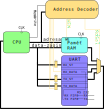
\includegraphics[width=\textwidth]{UART-cz.pdf}
\end{column}
\end{columns}

\end{frame}


\begin{frame}[fragile]
\frametitle{Sériový port v QtRvSim}

\begin{minted}[fontsize=\footnotesize]{gas}
.equ SERIAL_PORT_BASE,   0xffffc000 
#base address of QtRVSim serial port

.equ SERP_RX_ST_REG,       0xffffc000  #Receiver status register
.equ SERP_RX_ST_REG_o,     0x0000      #Offset of RX_ST_REG
.equ SERP_RX_ST_REG_READY_m, 0x1 #Data byte is ready to be read
.equ SERP_RX_ST_REG_IE_m,    0x2 #Enable Rx ready interrupt

.equ SERP_RX_DATA_REG,   0xffffc004 #Received data byte in 8 LSB bits
.equ SERP_RX_DATA_REG_o,   0x0004   #Offset of RX_DATA_REG

.equ SERP_TX_ST_REG,     0xffffc008 #Transmitter status register
.equ SERP_TX_ST_REG_o,     0x0008   #Offset of TX_ST_REG
.equ SERP_TX_ST_REG_READY_m,  0x1 #Transmitter can accept next byte
.equ SERP_TX_ST_REG_IE_m,     0x2 #Enable Tx ready interrupt

.equ SERP_TX_DATA_REG,   0xffffc00c #Write word to send 8 LSB bits
.equ SERP_TX_DATA_REG_o,   0x000c   #Offset of TX_DATA_REG
\end{minted}
\end{frame}

\begin{frame}[fragile]
\frametitle{Příklad vyslání znaku}

\begin{minted}[fontsize=\footnotesize]{gas}
write:
    li   a0, SERIAL_PORT_BASE # a0 ukazuje na zacatek pameti UART
    la   a1, text_1           # nacti ukazatel na retezec
next_char:
    lb   t1, 0(a1)            # nacti znak k odeslani
    beq  t1, zero, end_char   # 0 ukoncuje retezec
    addi a1, a1, 1            # posun ukazatel
tx_busy:
    lw   t0, SERP_TX_ST_REG_o(a0)       # zjisti statu odesilaci fronty
    andi t0, t0, SERP_TX_ST_REG_READY_m # vymaskuj bit READY
    beq  t0, zero, tx_busy    # pokud neni volno v UARTU cekej zkus to znovu
    sw   t1, SERP_TX_DATA_REG_o(a0) # je volno - zapis bajt
    j    next_char            # posli dalsi znak
end_char:
    ebreak                    # ukonci program

    .data
text_1:
    .asciz  "Hello world.\n"  # retezec ukonceny 0
\end{minted}

\end{frame}

\begin{frame}[fragile]
\frametitle{Příklad přijetí znaku}

\begin{minted}[fontsize=\footnotesize]{gas}
gets: li   a0, SERIAL_PORT_BASE # a0 ukazuje na zacatek pameti UART
    la   a1, text_1           # nacti ukazatel na buffer
    addi t2, zero, 40
next_char:
rx_not_ready:
    lw   t0, SERP_RX_ST_REG_o(a0)       # zjisti statu prijimaci fronty
    andi t0, t0, SERP_RX_ST_REG_READY_m # vymaskuj bit READY
    beq  t0, zero, rx_not_ready    # pokud neni znak UARTU cekej zkus to znovu
    lw   t1, SERP_RX_DATA_REG_o(a0) # je znak - precti ho a tim odstran
    sb   t1, 0(a1)            # uloz znak do bufferu
    addi t1, t1, -13          # test je to novy radek?
    beq  t1, zero, end_char   # ukoncuje cteni
    addi a1, a1, 1            # posun ukazatel
    addi t2, t2, -1            # kontroluj kolik muzeme nacist
    bne  t2, zero, next_char
end_char:
    ebreak                    # ukonci program
    .data
text_1:
    .word 0,0,0,0,0,0,0,0,0,0
\end{minted}
\end{frame}



\begin{frame}
\frametitle{QtRvSim Terminal -- serial port}
\begin{center}
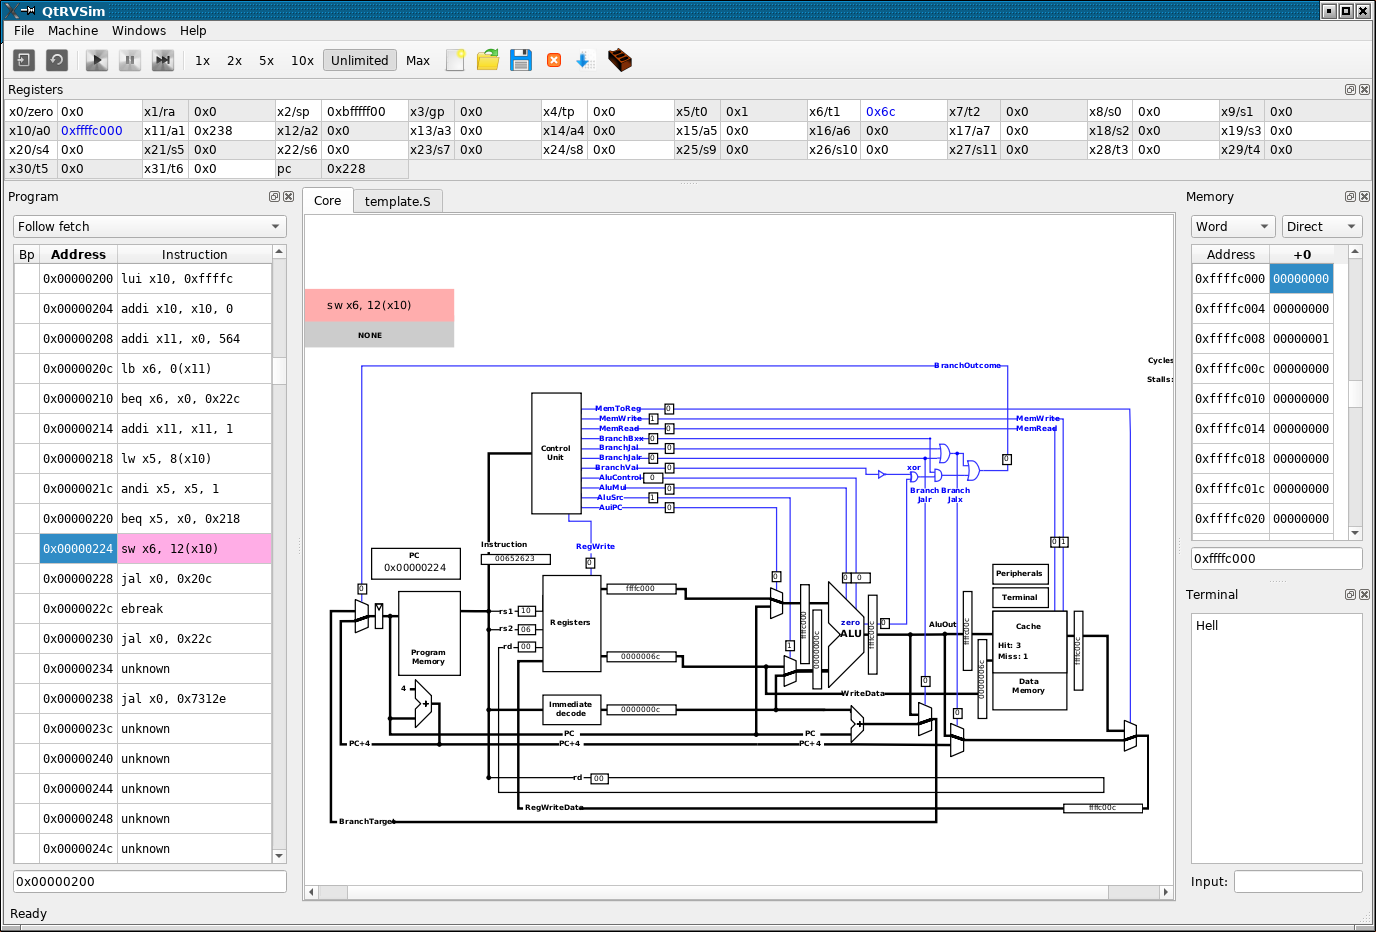
\includegraphics[width=0.8\textwidth]{fig/QtRvSim-serial-normal.png}
\end{center}
\end{frame}

\begin{frame}
\frametitle{QtRvSim Terminal -- serial port}
\begin{center}
Zřetězený procesor -- pipelined verze
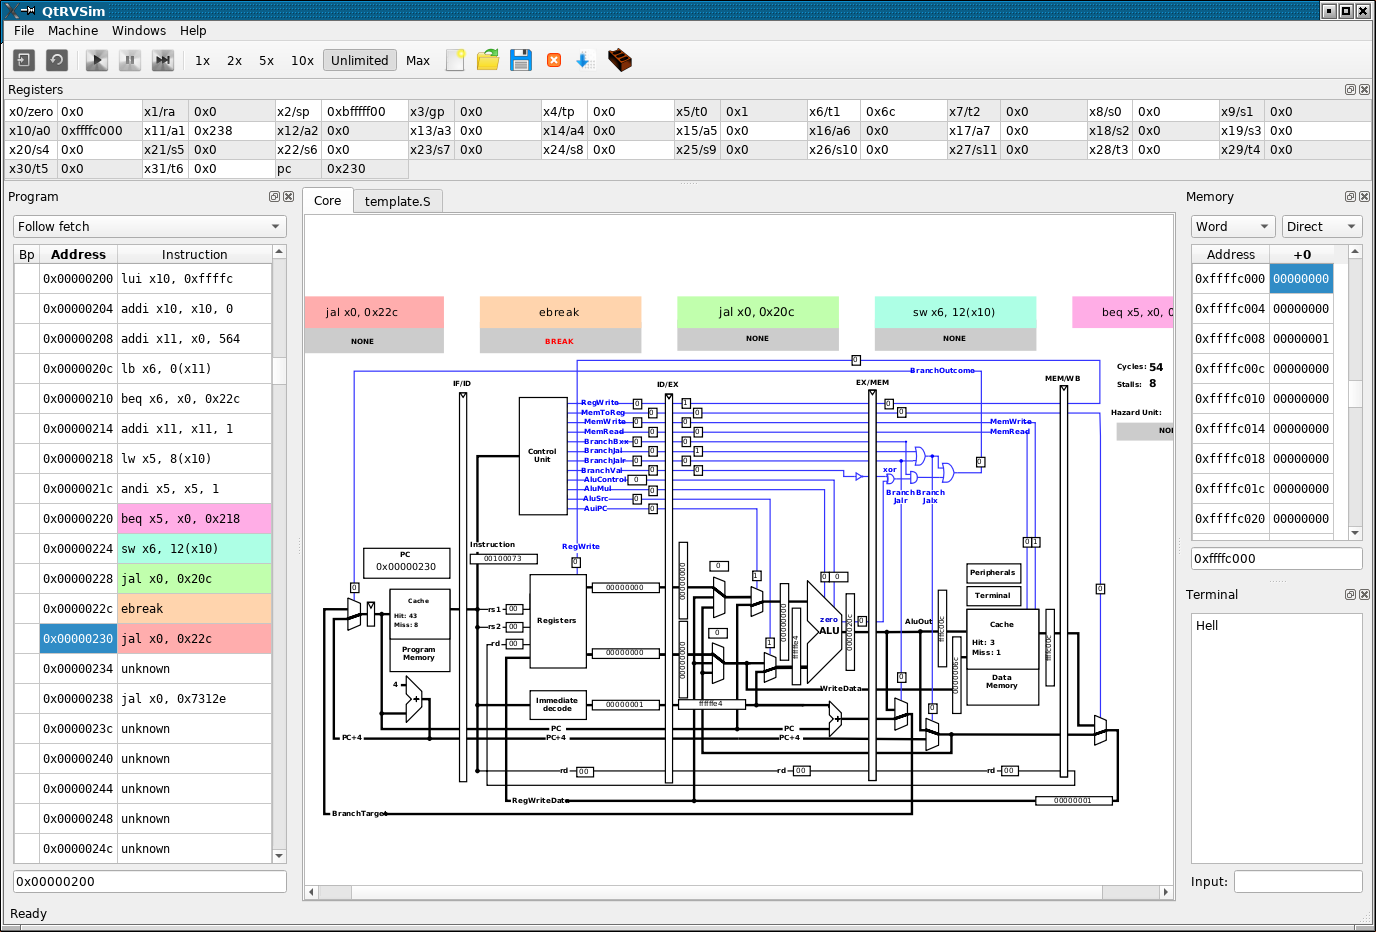
\includegraphics[width=0.8\textwidth]{fig/QtRvSim-serial-pipeline.png}
\end{center}
\end{frame}

\begin{frame}
\frametitle{Shrnutí komunikace periferií}

\begin{itemize}
\item uvedený způsob komunikace je tzv. polling
\begin{itemize}
\item program se neustále dotazuje, zda se něco nezměnilo, nepřišel znak, nebo se uvolnila odesílací fronta
\item toto je velmi neefektivní, zatěžuje zbytečně CPU, které by mohlo dělat něco užitečného
\end{itemize}
\item na přednášce 9 bude využití přerušení
\begin{itemize}
\item program může dělat něco jiného, přerušení nastane, pokud je povoleno a změní se stav periférie
\item při přerušení se začne provádět jiný program, který zjistí, jaká událost se stala a zpracuje ji
\item informace o tom co se stalo předá programu pomocí synchronizačních prostředků (bude v podrobně v předmětu OSY)
\end{itemize}
\end{itemize}

\end{frame}



\section{Sběrnice}

\begin{frame}
\frametitle{Stručná historie vnitřních sběrnic}

\begin{itemize}
\item ISA – starší typ pasivní sběrnice, šířka 8 nebo 16 bitů, přenosová rychlost maximálně 8 MB/s
\item PCI – novější typ „inteligentní“ sběrnice, šířka 32 nebo 64 bitů, burst režim, přenosová rychlost až 530 MB/s
\item AGP – jednoúčelová sběrnice určená pro připojení grafického karty přes severní můstek k CPU, přenosová rychlost 260 MB/s – 2 GB/s
\item PCI-Express (PCIe) – nová sériová implementace sběrnice PCI
\end{itemize}
\end{frame}


\begin{frame}
\frametitle{Topologie sběrnic}
\begin{center}
Sdílená sběrnice (např. PCI)
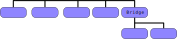
\includegraphics[width=0.8\textwidth]{shared_bus.pdf}
\end{center}

\begin{center}
Spojení peer-to-peer s využitím switch (např. PCIe, USB)
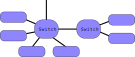
\includegraphics[width=0.65\textwidth]{switch_bus.pdf}
\end{center}
\end{frame}

\begin{frame}
\frametitle{PC sběrnice}
\begin{center}
Stará architektura Pentium 4 (90. léta minulého století)
\end{center}

\begin{columns}
\begin{column}{0.5\textwidth}
Severní můstek je připojen přímo k CPU a nejrychlejším periferiím -- paměti a grafické kartě
\bigskip

Jižní můstek komunikuje je připojen k severnímu a má síťové karty, HDD, PCI sloty.

\bigskip
Nejpomalejší periferie jako Floppy Disk, nebo sériová a paralelní port (tiskárny) bývají připojeny přes další můstky.
\end{column}
\begin{column}{0.5\textwidth}  
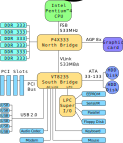
\includegraphics[width=\textwidth]{pentium4.pdf}
\end{column}
\end{columns}
\end{frame}

\begin{frame}
\frametitle{PC sběrnice}

\begin{center}
Moderní s ovladačem paměti na čipu.
\end{center}

\begin{columns}
\begin{column}{0.4\textwidth}
Severní můstek se stal součástí procesoru.

\bigskip
Jižní můstek komunikuje přímo s procesorem.

\bigskip
Většina periferií je připojena přes USB.
\end{column}
\begin{column}{0.6\textwidth}  
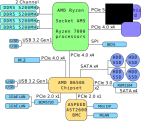
\includegraphics[width=\textwidth]{amd_am5.pdf}
\end{column}
\end{columns}
\end{frame}

\begin{frame}
\frametitle{PCI}

Sběrnice PCI je řízena hodinami. 

Pro správnou činnost je nutná co nejpřesnější synchronizace podle vysílaných hodin.

Signály označené \# jsou negované, protože sestupná hrana je rychlejší.

\begin{center}  
\includegraphics[width=0.7\textwidth]{PCI_clock.pdf}
\end{center}
\end{frame}

\begin{frame}
\frametitle{PCI architektura}

\begin{columns}
\begin{column}{0.35\textwidth}
Signál IDSEL je pouze pro inicializaci, zjištění, jaké zařízení je připojeno.

\bigskip
AD je 32 signálů používaných pro adresu a pro data

\bigskip
C/BE jsou 4 bity příkazu

\bigskip
CTRL jsou bity řídicí průběh přenosu
\end{column}
\begin{column}{0.6\textwidth}  
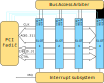
\includegraphics[width=\textwidth]{PCI_arch.pdf}
\end{column}
\end{columns}

\end{frame}


\begin{frame}
\frametitle{PCI přenos dat -- write}

\begin{itemize}
\item Přenos začíná iniciátor tím, že požádá arbitra o přidělení sběrnice
\begin{itemize}
\item Pokud o sběrnici požádá více zařízení současně, arbitr musí jejich žádosti seřadit a povolit najednou pouze jeden přenos
\end{itemize}
\item Iniciátor začne vysílání nastavením adresy cílové periférie na AD sběrnici a nastavením příznaku FRAME -- rámec přenosu a bitů cmd
\end{itemize}

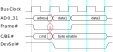
\includegraphics[width=0.8\textwidth]{PCI_write1.pdf}

\end{frame}

\begin{frame}
\frametitle{PCI přenos dat -- write}

\begin{itemize}
\item Periférie, která rozpozná svoji adresu nastaví DevSel na 1
\item Pokud je cílová periferie (Target) připravena přijmout data, nastaví TRDY na 1. 
\item Pokud je iniciátor připraven vyslat data, nastaví IRDY na 1
\end{itemize}

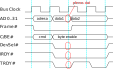
\includegraphics[width=0.8\textwidth]{PCI_write2-cz.pdf}

\end{frame}


\begin{frame}
\frametitle{PCI přenos dat -- write}

\begin{itemize}
\item Pokud by cílová periférie nebyla připravena, tak shodí příznak TRDY na 0
\item Pokud by iniciátor nebyl připraven dát data na sběrnici, shodí IRDY na 0 
\item Pokud je TRDY nebo IRDY na 0, pak je přenos dat pozastaven-
\end{itemize}

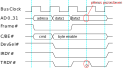
\includegraphics[width=0.8\textwidth]{PCI_write3-cz.pdf}

\end{frame}


\begin{frame}
\frametitle{PCI přenos dat -- write}

\begin{itemize}
\item Vyslání posledních dat je indikováno shozením příznaku FRAME na 0.
\item V našem případě byl přenos dat pozastaven, takže k přenosu posledních dat dojde až v dalším hodinovém cyklu.
\item Po ukončení přenosu se signály IRDY, TRDY a DEVSEL vrátí na 0 a sběrnice se uvolní pro další přenos.
\end{itemize}

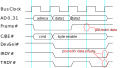
\includegraphics[width=0.8\textwidth]{PCI_write4-cz.pdf}

\end{frame}


\begin{frame}
\frametitle{PCI přenos dat -- read}

\begin{itemize}
\item Iniciátor žádá o data z cílové periférie.
\item Přenos dat je obdobný, ale nelze začít na následujícím hodinovém cyklu, protože se iniciátor musí od AD sběrnice odpojit a cílové zařízení se musí ke sběrnici připojit.
\end{itemize}

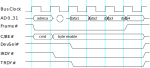
\includegraphics[width=0.8\textwidth]{PCI_read1.pdf}

\end{frame}


\begin{frame}
\frametitle{PCI shrnutí}

Nevýhody PCI sběrnice:
\begin{itemize}
\item Half--duplex nelze současně posílat data oběma směry, data se přesouvají pouze jedním směrem
\item Více zařízení na sběrnici -- pomalá periférie brzdí rychlé periférie, zvyšuje latency všech ostatních periférií
\item PCI sběrnice umožňuje pouze hodiny s 33 MHz, nebo 66 MHz
\begin{itemize}
\item To odpovídá 132MB/s nebo 264 MB/s pro 32 bitovou variantu
\item To odpovídá 264MB/s nebo 528 MB/s pro 64 bitovou variantu
\end{itemize}
\item PCI eXtended (PCI-X) sběrnice umožňuje hodiny až 133 MHz později maximálně 533 MHz
\begin{itemize}
\item To odpovídá přenosovým rychlostem 532MB/s až maximálně 4266 MB/s pro 64 bitovou variantu
\item PCI-X verze 2.0 s rychlostmi nad 133MHz nebyly moc rozšířené 
\end{itemize}
\item Konektor pro 32 bitovou verzi má 62 pinů -- tj. 124 signálů, pro 64 bitovou verzi je to dokonce 188 signálů  
\end{itemize}

\end{frame}


\begin{frame}
\frametitle{PCI Expres -- PCIe}

Zásadní nevýhoda paralelního přenosu je v potřebné kvalitě vodičů:
\begin{itemize}
\item i malé nepřesnosti v délce vodiče, kvalitě spojů vedou k rozdílným rychlostem šíření elektrického signálu
\item pro malé frekvence to není problém a zvyšující se frekvence zkracují délku vysílaných dat.
\item Podívejte se na animaci na https://cw.fel.cvut.cz/wiki/courses/b35apo/lectures/07/start
\end{itemize}
\bigskip

\begin{columns}[T]
\begin{column}{0.32\textwidth}  
frekvence $f$
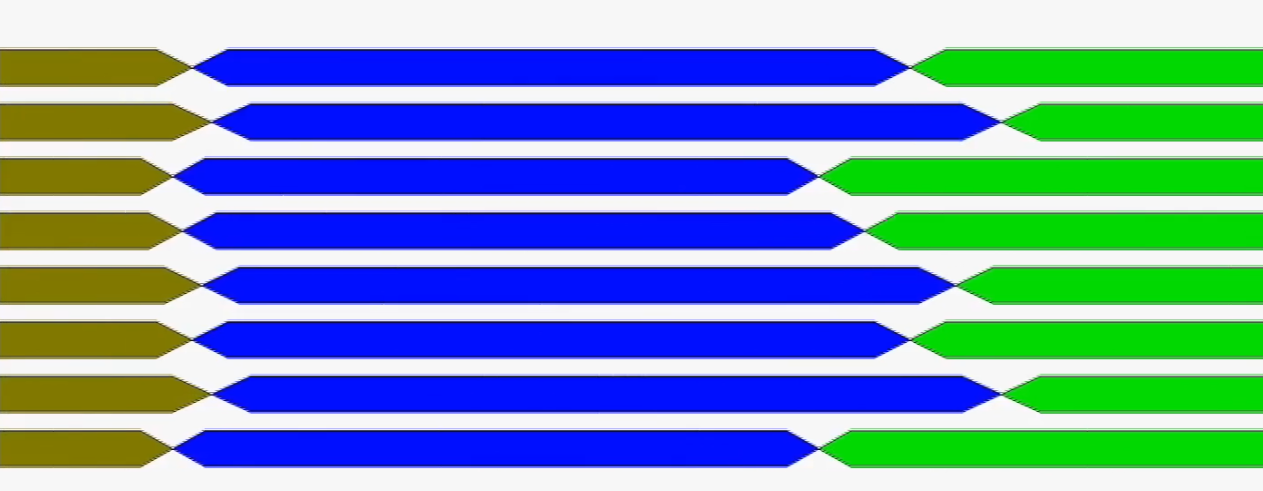
\includegraphics[width=\textwidth]{fig/freq1.png}
přenos bez problémů
\end{column}
\begin{column}{0.32\textwidth}  
frekvence $2\cdot f$
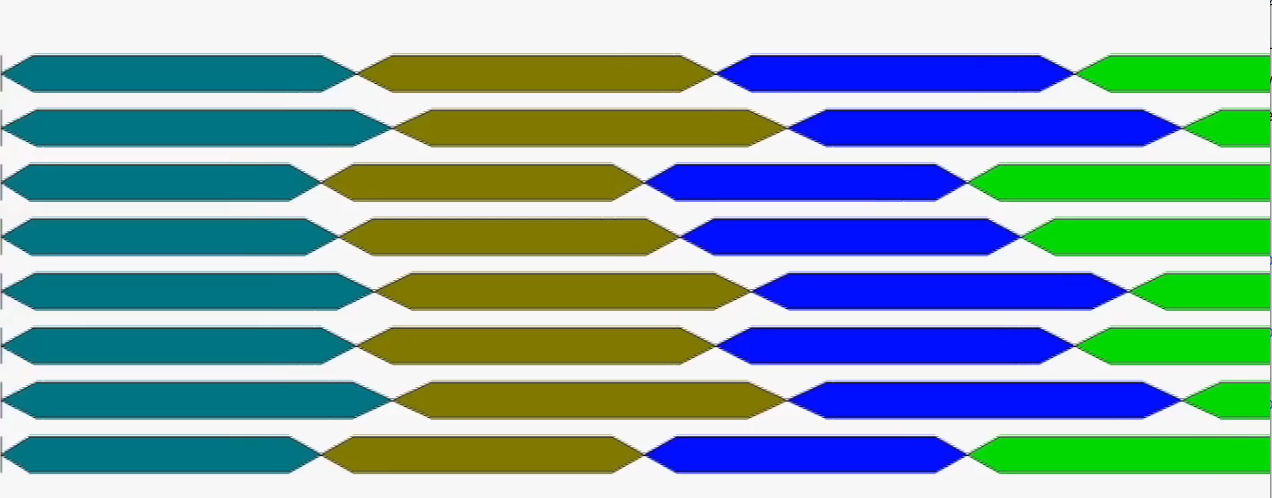
\includegraphics[width=\textwidth]{fig/freq2.png}
přenos na hraně spolehlivosti
\end{column}
\begin{column}{0.32\textwidth}  
frekvence $4\cdot f$
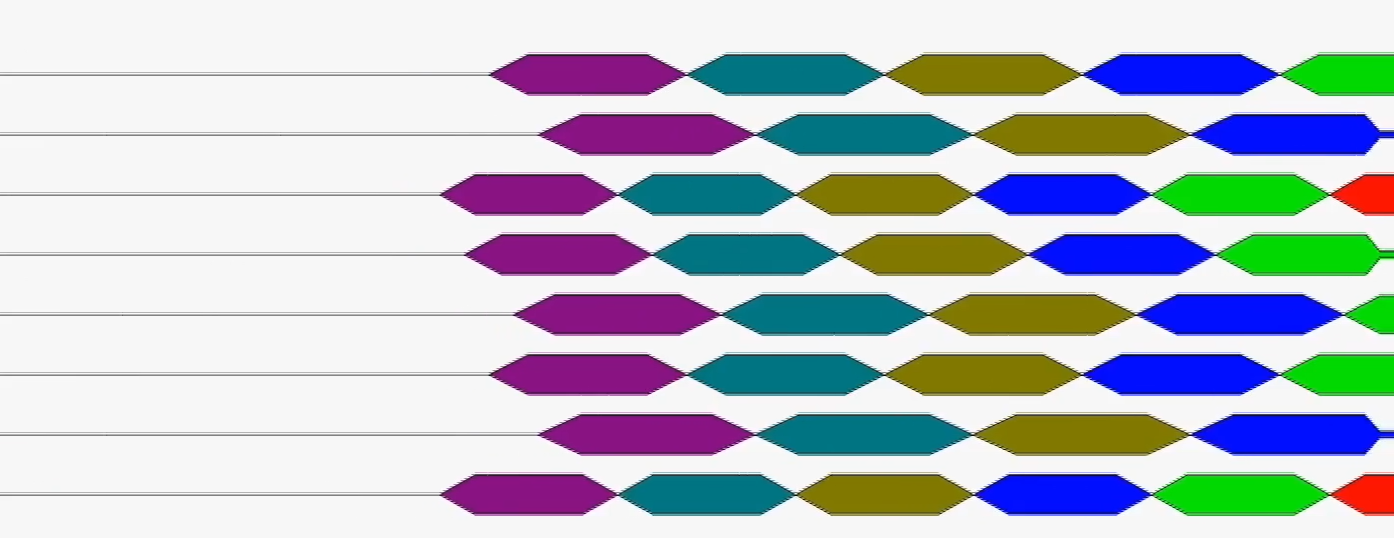
\includegraphics[width=\textwidth]{fig/freq4.png}
nelze v jeden okamžik detekovat výstupní data
\end{column}
\end{columns}

\end{frame}


\begin{frame}
\frametitle{PCIe rozdíly oproti PCI}

\begin{itemize}
\item PCIe je tzv. peer-to-peer, tedy signály jsou pouze mezi dvěma zařízeními.
\item PCIe je full-duplex tedy současně může probíhat přenos dat oběma směry.
\item Pro přenos jedním směrem se používá sériový způsob s dvěma vodiči a napětím mezi těmito vodiči.
\begin{itemize}
\item Tento způsob přenosu je méně náchylný na rušení než jedním vodičem vůči zemi.
\end{itemize}
\item PCIe může obsahovat více linek, ale přenos mezi linkami není synchronizován na úrovni bitů.
\item Konektory PCIe mají v nejjednodušší variantě pouze 18 pinů, 36 signálů z čehož 18 je uzemnění a napájení.
\end{itemize}

\end{frame}

\begin{frame}
\frametitle{PCIe sériový přenos}

\begin{itemize}
\item PCIe může využívat pro přenos různé rychlosti
\item Je nutné, aby přijímací strana mohla detekovat rychlost přenosu.
\item Problém je, pokud bajt obsahuje samé 0, nebo samé 1 nedochází ke změně signálu.
\item Řešením je, zakódovat bajt (8bitů) do 10bitů tak, aby celkový přenesený počet 0 a 1 byl stejný.
\end{itemize}

Kvíz: Kolik existuje různých 10-bitových čísel, které mají pět bitů 0 a pět bitů 1?
\begin{itemize}
\item[A] $2^5 \cdot 2^5 = 64$
\item[B] $5! \cdot 5! = 14400$
\item[C] ${10 \choose 5} = 252$
\item[D] $5! + 5! = 240$
\end{itemize}
\end{frame}


\begin{frame}
\frametitle{PCIe kódování 8b/10b}

\begin{itemize}
\item 8bitů, neboli 256 různých hodnot zakódujeme do 10bitového čísla, které má minimálně čtyři 0 a minimálně čtyři 1
\begin{itemize}
\item Takových 10-bitových čísel je již ${10 \choose 5} + 2\cdot {10 \choose 6}= 672$
\item Vybereme si takové, kde se hodně mění 1.
\end{itemize}
\item V kódovacích tabulkách je volnost vybrat si zda kód bude mít více 1, nebo více 0.
\item Ve skutečnosti se kód skládá ze dvou podkódů 5b/6b a 3b/4b.
\end{itemize}

\bigskip
tabulka kódu 3b/4b\phantom{xxxxx}{
\scriptsize
\begin{tabular}{|c|c|c|c|}\hline
\multicolumn{2}{|c|}{Input} & RD = −1 &	RD = +1 \\\hline
Code & HGF & \multicolumn{2}{c|}{f g h j} \\\hline
D.x.0 &000 &1011 & 0100\\\hline
D.x.1 &001 &\multicolumn{2}{c|}{1001}\\\hline
D.x.2 &010 &\multicolumn{2}{c|}{0101}\\\hline
D.x.A3 &011 &\multicolumn{2}{c|}{1100}\\
D.x.B3 &    &\multicolumn{2}{c|}{0011}\\\hline
D.x.4 &100 &1101 &0010\\\hline
D.x.5 &101 &\multicolumn{2}{c|}{1010}\\\hline
D.x.6 &110 &\multicolumn{2}{c|}{0110}\\\hline
D.x.P7 & 111 &1110 & 0001\\
D.x.A7 & &  0111 & 1000\\\hline
\end{tabular}
}
\end{frame}


\begin{frame}
\frametitle{PCIe ver. 1.x a 2.x}

Ver 1.x
\begin{itemize}
\item Frekvence přenosu je 2.5 GT/s (počet transferů za s)
\item Pro jeden bajt 8bitů je potřeba 10 transferů
\item Maximální přenosová kapacita je tedy 250 MB/s = $(2500 \cdot \frac{8}{10})$ Mb/s = $(2500 \cdot \frac{1}{10})$ MB/s
\item PCIe umožňuje pro jednu periferie mít 16 nezávislých linek, které se podělí o přenášená data -- nezávisle paralelně
\begin{itemize}
\item Maximální přenosová kapacita je $(16 \cdot 250)$ MB/s = $4$ GB/s
\end{itemize}
\end{itemize}

Ver 2.x
\begin{itemize}
\item Frekvence přenosu je 2.5 GT/s (počet transferů za s)
\item Pro jeden bajt 8bitů je potřeba 10 transferů
\item Maximální přenosová kapacita jedné linky (x1) je 500 MB/s
\item Maximální přenosová kapacita pro 16 linek (x16) je $(16 \cdot 500)$ MB/s = $8$ GB/s
\end{itemize}
\end{frame}

\begin{frame}
\frametitle{PCIe ver. 3.x, 4.x a 5.x}

Kódování 8b/10b je zbytečně neefektivní, zvolilo se kódování 128b/130b s obdobnými parametry.
\begin{itemize}
\item Ver 3.x 
\begin{itemize}
\item Frekvence přenosu je 8 GT/s (počet transferů za s)
\item Maximální přenosová kapacita je tedy skoro 985 MB/s = $(8000 \cdot \frac{128}{130})$ Mb/s = $(8000 \cdot \frac{16}{130})$ MB/s
\item Maximální přenosová kapacita pro x16 je $(16 \cdot 985)$ MB/s = $15.75$ GB/s
\end{itemize}
\item Ver 4.x 
\begin{itemize}
\item Frekvence přenosu je 16 GT/s (počet transferů za s)
\item Maximální přenosová kapacita je tedy skoro 1.97 GB/s = $(16000 \cdot \frac{16}{130})$ MB/s
\item Maximální přenosová kapacita pro x16 je $(16 \cdot 1.97)$ GB/s = $31.5$ GB/s
\end{itemize}
\item Ver 5.x 
\begin{itemize}
\item Frekvence přenosu je 32 GT/s (počet transferů za s)
\item Maximální přenosová kapacita je tedy skoro 3.94 GB/s = $(32000 \cdot \frac{16}{130})$ MB/s
\item Maximální přenosová kapacita pro x16 je $(16 \cdot 3.94)$ GB/s = $63$ GB/s
\end{itemize}
\end{itemize}

\end{frame}




\begin{frame}
\frametitle{PCIe topologie}

Komunikace po PCIe sběrnici se podobá komunikaci po síti (ethernet).
\begin{itemize}
\item Komunikace probíhá po paketech 
\begin{itemize}
\item POZOR -- režie paketů není započítána do maximální přenosové kapacity.
\item Každý paket má synchronizační hlavičku, adresu, data, crc -- obdobně jako v protokolu ethernet.
\end{itemize}
\item Využití přepínačů (switch) je podobné jako v síti
\begin{itemize}
\item Přepínače umožňují komunikovat pouze mezi dvěma zařízeními
\item Přepínače umí prioritizovat pakety -- výhodné pro snížení latence (použití paketů naproti tomu latenci zvyšuje)
\item Pomocí přepínačů lze zajistit automatickou detekci a konfiguraci připojených zařízení na obdobném principu, jako to dělal PCI sběrnice 
\end{itemize}
\end{itemize}

\end{frame}

\begin{frame}
\frametitle{Realita signálů sériové sběrnice}

Vysokorychlostní komunikace přináší mnoho různých problémů.

Vzhled signálů v závislosti na vzdálenosti

\begin{center}
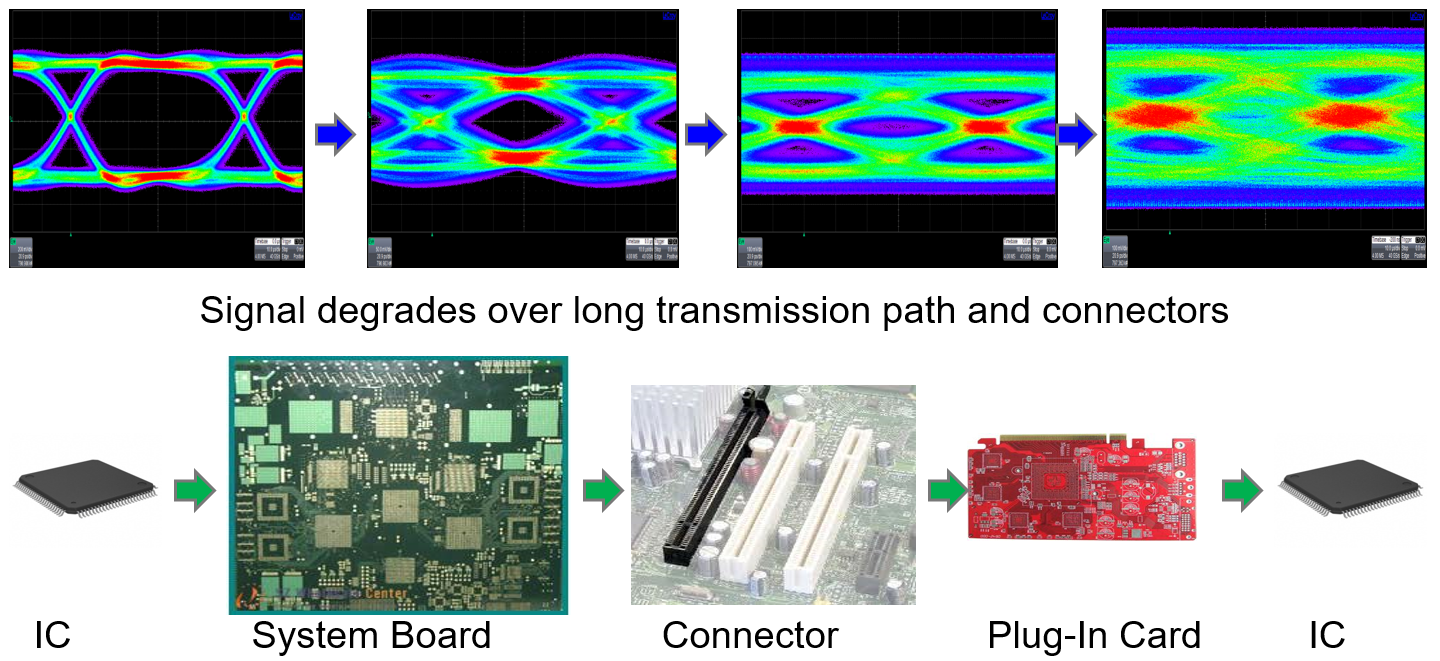
\includegraphics[width=0.8\textwidth]{fig/signals.png}
\end{center}

\end{frame}


\begin{frame}
\frametitle{Hard disky}

\begin{itemize}
\item Obdobný vývoj, který je u změny PCI na PCIe lze pozorovat i u disků.
\item PATA neboli Parallel ATA je paralelní připojení disku od roku 1984 pro první IBM PC/AT
\begin{itemize}
\item Název ATA znamená vlastně AT Attachment, AT je zkratka Advance Technology.
\item Také označován jako IDE, později Extended IDE (EIDE) Utra ATA (UATA) 
\item PATA je 16-bitový paralelní přenos dat mezi CPU a diskem
\item Ve své nejrychlejší variantě uměl přenášet až 133 MB/s 
\end{itemize}
\item SATA je sériová verze komunikace s diskem.
\begin{itemize}
\item V minimální variantě potřebuje pouze 7 vodičů, A+,A-, B+, B- a 3x zemění.
\begin{itemize}
\item SATA 1.0: 150 MB/s  (PATA:130MB/s)
\item SATA 2.0: 300 MB/s
\item SATA 3.0: 600 MB/s
\item SATA 3.2: about 2 GB/s
\end{itemize}
\end{itemize}
\end{itemize}
\end{frame}


\end{document}

